\documentclass[conference, spanish, english]{IEEEtran}
\IEEEoverridecommandlockouts
% The preceding line is only needed to identify funding in the first footnote. If that is unneeded, please comment it out.
\usepackage[T1]{fontenc}
\usepackage[utf8]{inputenc}
\usepackage{babel}
\usepackage{cite}
 \usepackage{booktabs}
\usepackage{amsmath,amssymb,amsfonts}
\usepackage{algorithmic}
\usepackage{graphicx}
\usepackage{textcomp}
\usepackage{float}
\usepackage{enumitem}
\usepackage{fancyhdr}
\usepackage{xcolor}
\def\BibTeX{{\rm B\kern-.05em{\sc i\kern-.025em b}\kern-.08em
    T\kern-.1667em\lower.7ex\hbox{E}\kern-.125emX}}

\fancypagestyle{plain}{%
    \fancyhf{} % Limpia los encabezados y pies de página
    \fancyfoot[R]{\thepage} % Coloca el número de página en la esquina derecha del pie de página
    \renewcommand{\headrulewidth}{0pt} % Elimina la línea horizontal del encabezado
}
\begin{document}

\title{Detección de sirenas para conductores con discapacidad auditiva con CNN
}

\author{
    \IEEEauthorblockN{
        Archibald Emmanuel Carrion Claeys\IEEEauthorrefmark{1},
        Fabián Vega Meza\IEEEauthorrefmark{2}, 
        Marlon Esteban Murillo Quesada\IEEEauthorrefmark{3} y 
        Edgar Casasola Murillo\IEEEauthorrefmark{4}
    }
    \IEEEauthorblockA{
        \textit{
        Escuela de Computación, Universidad de Costa Rica} \\
        San Jose, Costa Rica \\
        Email: 
        \IEEEauthorrefmark{1}archibald.carrion@ucr.ac.cr,  \IEEEauthorrefmark{2}fabian.vegameza@ucr.ac.cr, \IEEEauthorrefmark{3}marlon.murilloquesada@ucr.ac.cr, \IEEEauthorrefmark{4}edgar.casasola@ucr.ac.cr}
}

\maketitle
\thispagestyle{plain}
\pagestyle{plain}

\selectlanguage{spanish}

\setcounter{page}{1} % Inicia la numeración de páginas desde 1
\begin{abstract}

Este proyecto presenta el desarrollo de un sistema basado en redes neuronales convolucionales (CNN) para la detección de sirenas de ambulancia en entornos urbanos de San Jose, Costa Rica. Utilizando un enfoque que combina la recolección de datos en campo y fuentes de internet, se transforman los audios en espectrogramas para identificar los sonidos de sirenas. Se proponen tres arquitecturas de CNN para abordar este problema y se realiza una comparación entre ellas para destacar sus distintas características y desempeños en la detección de los sonidos de sirenas proporcionados.\\
\end{abstract}

\selectlanguage{english}
\begin{abstract}
This project presents the development of a system based on Convolutional Neural Networks (CNNs) for detecting ambulance sirens in urban environments in San Jose, Costa Rica. Using an approach that combines data collection in the field and from internet sources, audio is transformed into spectrograms to identify siren sounds. Three CNN architectures are proposed to address this problem, and a comparison is conducted among them to highlight their different characteristics and performances in detecting the provided siren sounds.
\end{abstract}

\selectlanguage{spanish}
\section{Justificación}

\IEEEPARstart{L}a detección de sirenas de ambulancia en entornos urbanos es crucial para la seguridad y la movilidad en las vías públicas, siendo aún más desafiante para las personas con discapacidad auditiva, quienes no pueden percibir estos sonidos a distancia sin visualizar las luces de emergencia. Este proyecto tiene como objetivo intentar abordar esta limitación mediante el desarrollo de una red neuronal convolucional capaz de identificar sonidos de ambulancia dado un audio, con intención de que futuros proyectos puedan implementarlo a un sistema físico accesible capaz de identificar y alertar visualmente sobre la presencia de ambulancias cercanas. En Costa Rica, donde se permite a las personas con discapacidad auditiva conducir, esta tecnología adquiere una relevancia adicional al proporcionar una herramienta esencial para mejorar su autonomía y seguridad durante situaciones de emergencia en las vías públicas.

\section{Objetivo general}
El objetivo general de esta investigación es desarrollar e implementar un sistema basado en inteligencia artificial capaz de detectar las sirenas de ambulancias costarricenses a partir de grabaciones de audios tomados en ambientes del área de San Jose. Además diseñar y crear un conjunto de datos para llevar a cabo la experimentación.

\section{Objetivos específicos}

\begin{itemize}
 \item Diseñar y crear un conjunto de datos conformado de sonidos grabados en Costa Rica para optimizar el rendimiento de nuestro sistema.
 \item Desarrollar tres arquitecturas de redes neuronales convolucionales para clasificar audios entre los que contienen sonido de sirenas de ambulancia y los que no.
 \item Evaluar el desempeño de tres arquitecturas diferentes planteadas de redes neuronales convolucionales
 \item Analizar posibles soluciones de mejora.\\
\end{itemize}

\section{Antecedentes}
La detección de sirenas en el tráfico urbano ha sido objeto de estudio de varias publicaciones debido a su impacto en la seguridad vial y la eficiencia en la respuesta de los servicios de emergencia. A continuación, se presenta un resumen de algunos avances importantes en esta área.

\begin{itemize}

\item \textbf{\cite{Dobre2015} R. A. Dobre et al., "Low Computational Method for Siren Detection,"  2015.}
Un sistema de asistencia a la conducción que pueda detectar el sonido de sirenas y advertir al conductor. Se propuso una solución de bajo costo, en la que los sonidos de sirenas son interpretados por un Filtro paso banda de múltiples entradas para detectar las frecuencias comunes de una sirena de ambulancia en Rumanía. Después se pasó por diferentes componentes analógicos para determinar si el sonido es de ambulancia. El sistema fue simulado utilizando MATLAB y SPICE, mostrando resultados prometedores en la detección eficiente de sirenas.

  
\item \textbf{\cite{Pramanick2021} D. Pramanik et al., "Deep learning based urban sound classification and ambulance siren detector using spectrogram" 2021.}
Este artículo describe el desarrollo de una arquitectura para la detección de sirenas de ambulancia y la clasificación de sonidos urbanos utilizando diversas transformaciones de sonido a imagen, como Mel-spectrogramas, Scalogramas y el método de descomposición de Fourier (FDM). Esta investigación analiza los efectos de las técnicas de aumento y preprocesamiento en la eficacia de la arquitectura desarrollada frente a modelos preentrenados. El rendimiento del algoritmo propuesto se probó en el conjunto de datos Urbansound8K para la clasificación de sonidos urbanos y en un conjunto de datos de múltiples fuentes para la detección de sirenas de ambulancia. La CNN propuesta alcanzó una precisión del 89.66 en la clasificación de sonidos urbanos y del 99.35 en la detección de sirenas



\item \textbf{\cite{Fatimah2020} Fatimah et al., "An Automatic Siren Detection Algorithm Using Fourier Decomposition Method and MFCC"
 2020.}
Se propone un algoritmo automático para la detección de sirenas utilizando la descomposición de Fourier y los coeficientes de cepstrum de frecuencia mel (MFCC). Este sistema emplea algoritmos de aprendizaje supervisado, como SVM(Máquinas de vectores de soporte) y árboles bagged ensemble, para entrenar modelos que distinguen las sirenas de otros ruidos de tráfico en la India.

\end{itemize}

\section{Marco Teórico}
 
\begin{center}
    A. Descripción de una CNN
\end{center}

Las CNN ~\cite{Ketkar2021} son esencialmente una red neuronal que emplea la operación de convolución (en lugar de una capa completamente conectada) como una de sus capas, lo cual permite aprender características espaciales y temporales dentro de los datos. Esta estructura se inspira en la capacidad del sistema nervioso biológico para detectar y procesar patrones en imágenes de manera eficiente y robusta.
\begin{center}
    B. Elementos de una CNN
\end{center}

Las CNN están compuestas por tres capas principales: la capa de Convolución, la capa de pooling o agrupación, y la capa totalmente conectada.

\begin{itemize}
 \item \textbf{Capa de Convolución:} La capa de convolución se utiliza para extraer características locales relevantes de las imágenes, como bordes, texturas y patrones de color. Esta emplea filtros o kernels que exploran la imagen y capturan patrones específicos mediante operaciones de multiplicación y suma de elementos, similar a detectar cambios rápidos de intensidad de color en un área específica de la imagen.
 
 \item \textbf{Capa de Pooling:} La capa de pooling tiene como objetivo reducir la dimensionalidad de la representación de la imagen mientras conserva las características más importantes para el análisis y reconocimiento de patrones. La imagen se divide en regiones y se aplica una operación de agregación como el máximo o el promedio sobre cada región, preservando características críticas como formas y texturas sin perder detalles importantes. Esta capa reduce la cantidad de datos a procesar, lo que disminuye el costo computacional y la complejidad del modelo.
 
 \item \textbf{Capa totalmente conectada:} En la capa totalmente conectada, todas las características aprendidas por las capas de convolución y pooling se utilizan para realizar la clasificación o regresión final de la imagen. Cada unidad neuronal en esta capa está conectada a todas las unidades de la capa anterior (generalmente la última capa de pooling), permitiendo que cada neurona considere todas las características extraídas en las etapas anteriores para hacer predicciones finales sobre la imagen.
 
\end{itemize}


\begin{center}
    C. Tensorflow
\end{center}
\cite{pang2020} Tensorflow es una plataforma creada por Google para desarrollar proyectos de aprendizaje automático, utilizando una serie de herramientas para entrenar y ejecutar modelos de redes neuronales. Esta biblioteca contiene una amplia variedad de herramientas para implementar redes convolucionales. Cuenta con funcionalidaddes usadasen el proyecto como, capas convolucionales, de pooling y totalmente conectada. Las capas convolucionales se implementan mediante la clase tf.keras.layers.Conv2D, que es parte del módulo Keras de TensorFlow. Esta clase permite definir y configurar capas convolucionales de manera sencilla. Se especifica el número de filtros (o kernels) y el tamaño del kernel. Además de la función de activación aplicada en ella.

\begin{itemize}
 \item \textbf{Función de activación:} Estas funciones transforman la salida de una neurona, permitiendo que el modelo capture patrones no lineales. Tres de las funciones de activación más utilizadas son Sigmoid, ReLU (Rectified Linear Unit) y tanh.
 \item \textbf {Rectified Linear Unit(ReLU):} Esta función genera una salida igual a cero cuando la entrada sea negativa, y una salida igual a la entrada cuando esta sea positiva. Además, no cuenta con saturación, lo que causa que converja más rápidamente y sea computacionalmente poco costosa.
 \item \textbf {Tangente Hiperbólica (tanh):} La función tanh produce valores en el intervalo de -1 a +1. Esta si cuenta con mayores problemas de saturacion que relu, pero tiene mejor rendimiento con entradas negativas que ReLu. 
 \item \textbf {Función de Activación Sigmoid
:} Los valores de salida de la función sigmoid están en el intervalo de 0 a 1. Esto convierte cualquier entrada en una probabilidad, lo que ayuda en la clasificación binaria. Esta función es continua, lo que facilita la propagación de los gradientes durante el entrenamiento.

\end{itemize}

\begin{center}
    D. Espectrograma
\end{center}

Un espectrograma ~\cite{paz2020procesamiento} es una herramienta básica de representación que se utiliza para el análisis de una señal eléctrica, de comunicación, o audiovisual, en la que se visualiza la energía del contenido frecuencial de la señal, según va variando a lo largo del tiempo. En otras palabras, es una representación visual o una conversión a imagen de la intensidad de las frecuencias de una señal de audio a lo largo del tiempo. 

\begin{figure}[H]
\centering
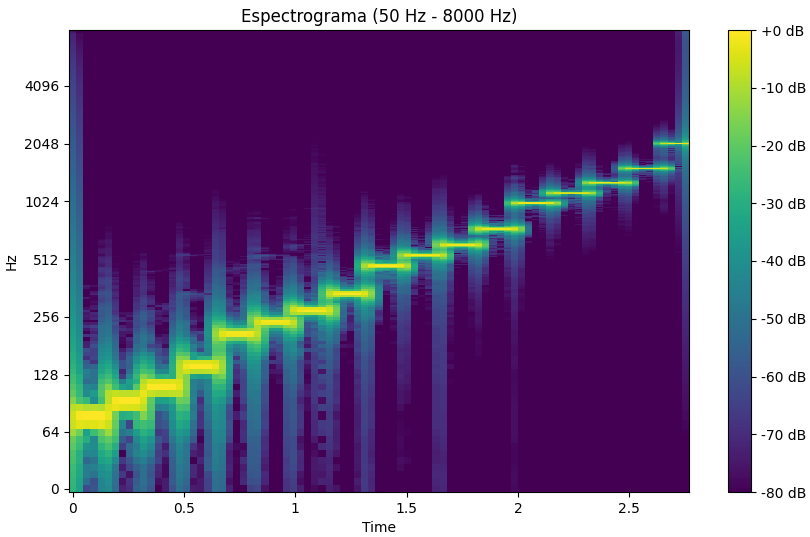
\includegraphics[width=0.48\textwidth]{espectrogramas/espectrograma_ejemplo.png}
\caption{Ejemplo de un espectrograma..}
\label{fig:ejemploEspectograma}
\end{figure}

La representación se realiza en tres dimensiones: temporal (en el eje x), frecuencial (en el eje y) y amplitud (representada por el color). En la figura~\ref{fig:ejemploEspectograma} se muestra un ejemplo de espectrograma que representa gráficamente una escala musical ascendente.

\section{Metodología}
\begin{center}
    A. Conjunto de datos para el entrenamiento
\end{center}

Para llevar a cabo el proyecto, primero se creó un conjunto de datos para el entrenamiento de la red neuronal. Se obtuvieron audios a partir de varias grabaciones de campo que se hicieron en las vías públicas del área de San Jose, además de varios videos de YouTube que contenían sirenas de ambulancia y sonidos ambientales de zonas urbanas costarricenses.\cite{likebupt_smote} Se recolectaron muchos mas audios sin sirenas, por lo que se aplico la tecnca de SMOTE en la cual se hace un sobremuestreo de minorías sintéticas para aumentar el número de casos de un conjunto de datos de forma equilibrada.
Estos audios fueron segmentados en fragmentos de 3 segundos en formato .wav (waveform audio format). Los fragmentos fueron clasificados en dos categorías: sonidos de ambulancia y sonidos ambientales sin sirenas. Al momento de entrenar y probar los modelos, se usaron 2 subdivisiones aleatorias del conjunto de datos: una primera subdivisión para el entrenamiento del modelo, y una segunda para la prueba del modelo.

\begin{center}
    B. Preprocesamiento de los datos
\end{center}

Los datos se pasaron por un proceso de estandarización para poderlos ingresar a las CNN de manera correcta. A estos audios se les aplicó una operación de preprocesamiento en la cual los audios se normalizaron a una frecuencia de 16 kHz y se convirtieron a formato mono de un solo canal. Posteriormente, los audios de entrenamiento procesados fueron convertidos en espectrogramas.

\begin{figure}[H]
\centering
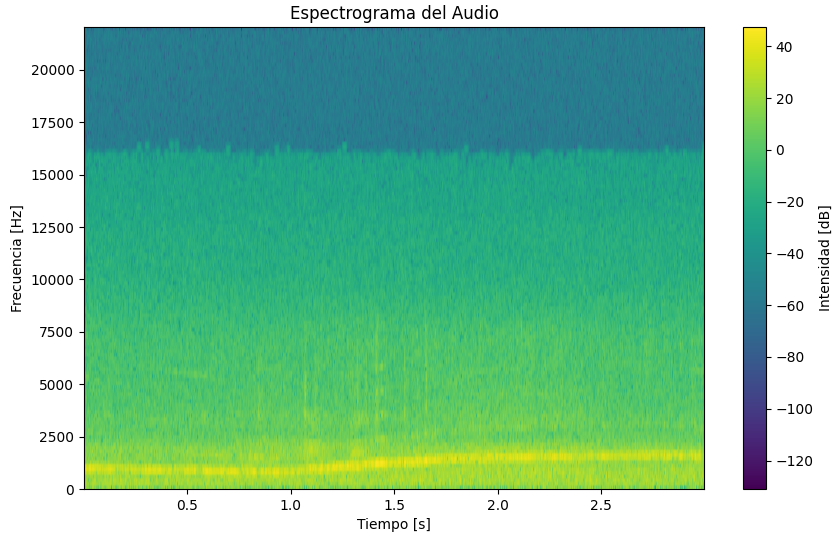
\includegraphics[width=0.48\textwidth]{espectrogramas/espectrograma.png}
\caption{Espectrograma de un sonido de sirena.}
\label{fig:espectograma}
\end{figure}


En la figura~\ref{fig:espectograma}, se muestra el espectograma de uno de los audios utilizados para el entrenamiento. La línea amarilla que aparece en la parte inferior del espectrograma representa la sirena de una ambulancia. Podemos observar que es la señal con mayor amplitud, lo que se evidencia por su color amarillo intenso.

\begin{center}
    C. Entrenamiento del Modelo
\end{center}

Después de realizar todos los preprocesamientos en los datos, se procede a entrenar las redes neuronales convolucionales utilizando el conjunto de datos preparado. Se exploraron tres arquitecturas con diferentes parámetros en sus capas, incluyendo variaciones en las funciones de activación como ReLU y tanh, además de la adición de capas de pooling en la red.

\begin{figure}[H]
\centering
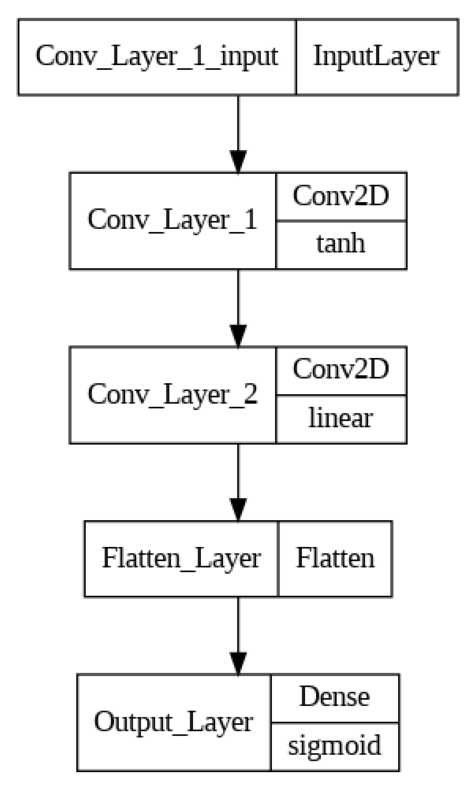
\includegraphics[width=0.25\textwidth]{architecture/architecture_2.png}
\caption{Arquitectura de la primera red}
\label{fig:arquitectura1}
\end{figure}

La primera arquitectura (ver figura~\ref{fig:arquitectura1}) presenta una capa de entrada, dos convolucionales con función de activacion tanh, seguido de una capa de aplanamiento (o flatten layer en inglés) que se usa para convertir una matriz multidimensional en un vector unidimensional. Dentro de las capas convolucionales, se utilizan 32 filtros en la primera y 64 en la segunda. Este proceso es esencial cuando se pasa de las capas convolucionales a las capas densas, tal como es nuestra capa de salida. 


\begin{figure}[H]
\centering
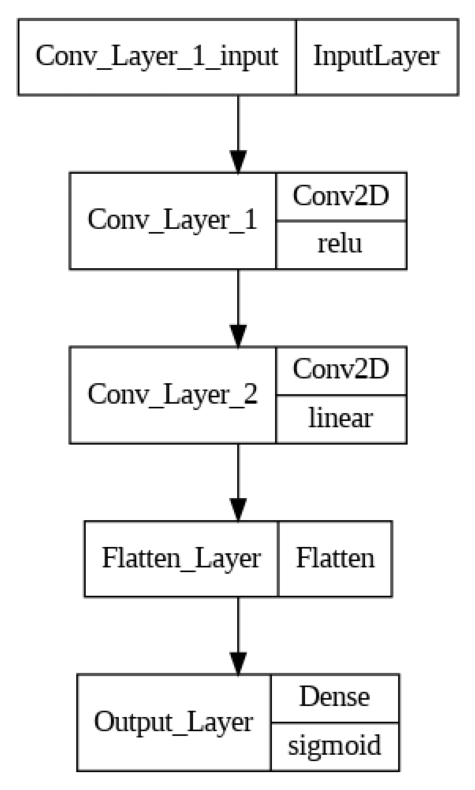
\includegraphics[width=0.25\textwidth]{architecture/architecture_3.png}
\caption{Arquitectura de la segunda red}
\label{fig:arquitectura2}
\end{figure}

La segunda arquitectura (ver figura~\ref{fig:arquitectura2}) sigue un formato bastante similar al primero ya que tambien presenta una capa de entrada, dos convolucionales, seguido de una capa de aplanamiento que se usa para convertir una matriz multidimensional en un vector unidimensional. La mayor diferencia es que las capas convolucionales usan la funcion de activacion relu, la cual tiende a ser menos compleja computacionalmente hablando. 


%En la primera se aplicaron dos capas de convolucion,la primera con 32 filtros de profundidad y cada uno de tamaño 3x3 pixeles con la funcion de activacion tanh. La segunda capa se le cambiaron los filtros a 64, y manteniendo los demas atributos. Despues se efectua una capa de aplanamiento para traducir los resultados de las capas en 2d a un vector final. Tras eso se agrega una capa final de densidad para clasificación binaria entre sirena o no sirena.

%La segunda arquitectura sigue el mismo formato que la anterior, pero esta vez, probando con la funcion de activacion ReLu. 

\begin{figure}[H]
\centering
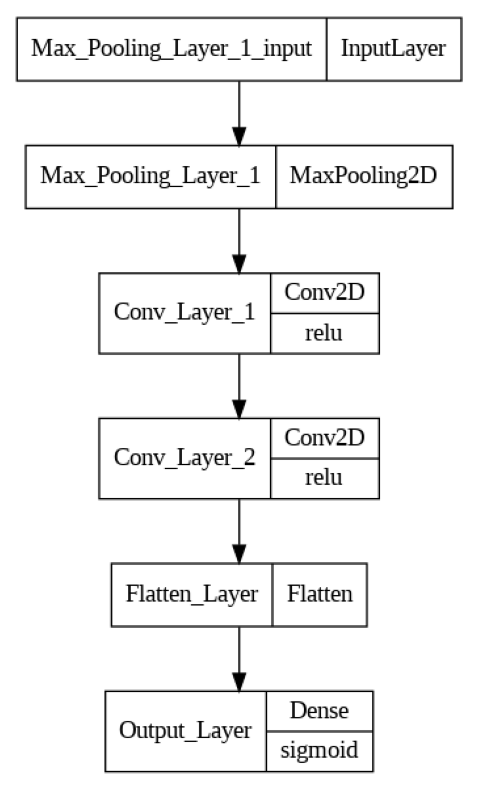
\includegraphics[width=0.25\textwidth]{architecture/architecture_4.png}
\caption{Arquitectura de la tercera red}
\label{fig:arquitectura3}
\end{figure}

La tercera arquitectura (ver figura~\ref{fig:arquitectura3}) sigue un patrón similar a la arquitectura analizada previamente, con la diferencia de que previo a las capas de convolución se hace una operación en la cual se extrae la información más representativa: la matriz. Esto se hace por medio de la capa de MaxPooling, la cual selecciona los valores más altos de una entrada, para crear una segunda más reducida.

\section{Resultados}

Todos los resultados presentados en el cuadro ~\ref{tab:tiemposEjecucionComparacion}. Fueron obtenidos con 5 epocas.

\begin{table}[H]
\caption{Tiempos de ejecución de cada arquitectura.\label{tab:tiemposEjecucionComparacion}}

\begin{tabular}{lrr}
\toprule 
 
\cmidrule{2-3} 
 &  \multicolumn{1}{c}{Tiempos de entrenamiento}
  & \multicolumn{1}{c}{Tiempos de prueba}
 \tabularnewline
\midrule 

Arquitectura 1 & $812.339$ & $27.761$  \tabularnewline
\midrule

Arquitectura 2 & $771.902$ & $27.827$  \tabularnewline
\midrule

Arquitectura 3 & $191.327$ & $21.768$  \tabularnewline
\midrule
\bottomrule
\end{tabular}
\end{table}

\begin{center}
    A. Arquitectura 1
\end{center}
Al entrenar la primera arquitectura propuesta, se nota que presenta una matriz de confusión casi perfecta, con únicamente dos falsos positivos. Se puede apreciar lo anterior viendo la matriz de la figura~\ref{fig:MatrizArqui1} .


\begin{figure}[H]
\centering
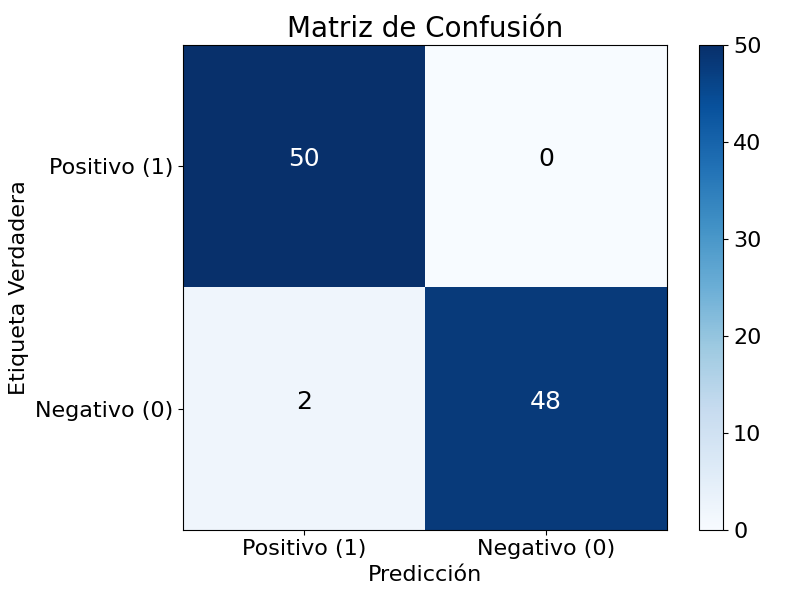
\includegraphics[width=0.48\textwidth]{training_plots/plot_architecture_2/confusion_matrix.png}
\caption{Matriz de Confusión generada tras probar la primera Arquitectura.}
\label{fig:MatrizArqui1}
\end{figure}


Es importante notar que el entrenamiento (ver cuadro ~\ref{tab:tiemposEjecucionComparacion}) dura 812 segundos, además para las pruebas dura un total de 27.7 segundos. Por lo que, por complejidad temporal, es el tercero mejor.

\begin{figure}[H]
\centering
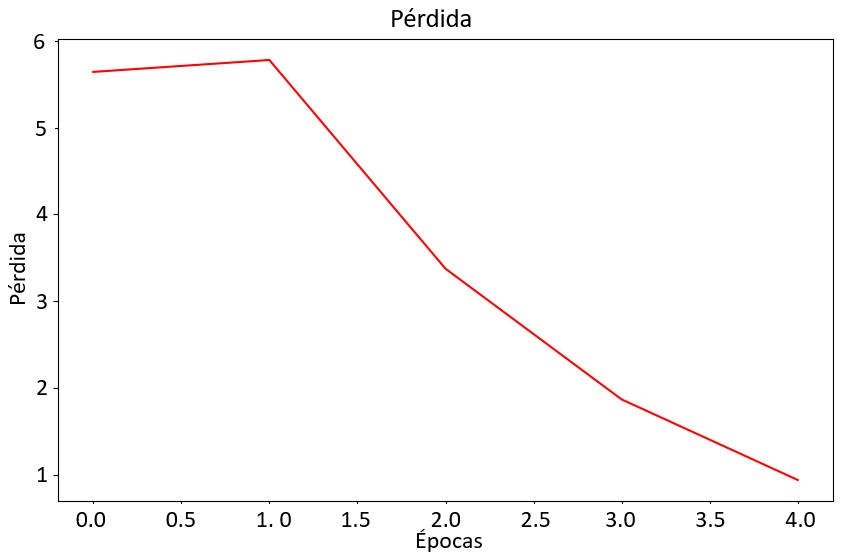
\includegraphics[width=0.48\textwidth]{training_plots/plot_architecture_2/loss_plot.png}
\caption{Grafo de pérdida generado durante el entrenamiento de nuestra primera Arquitectura.}
\label{fig:perdidaArqui1}
\end{figure}


\begin{figure}[H]
\centering
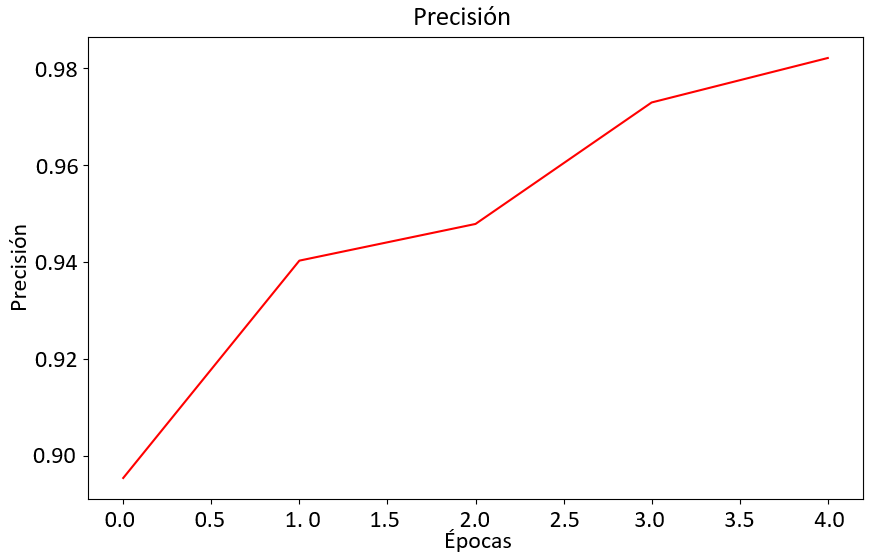
\includegraphics[width=0.48\textwidth]{training_plots/plot_architecture_2/precision_plot.png}
\caption{Grafo de precisión generado durante el entrenamiento de nuestra primera Arquitectura.}
\label{fig:precisionArqui1}
\end{figure}


\begin{figure}[H]
\centering
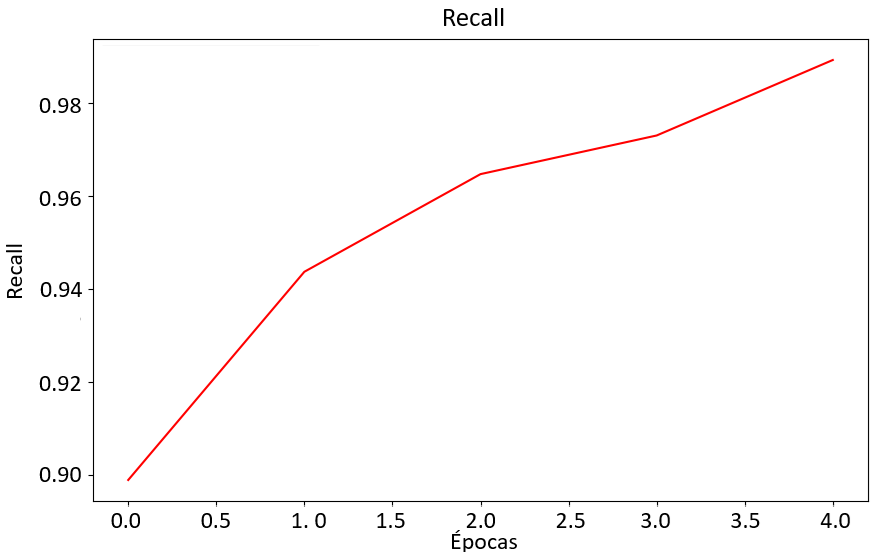
\includegraphics[width=0.48\textwidth]{training_plots/plot_architecture_2/recall_plot.png}
\caption{Grafo de recall generado durante el entranamiento de nuestra primera Arquitectura.}
\label{fig:recallArqui1}
\end{figure}



\begin{center}
    B. Arquitectura 2
\end{center}
Al entrenar la segunda arquitectura propuesta, se puede notar que también se obtuvo una matriz de confusión casi perfecta (ver figura ~\ref{fig:MatrizArqui2}) , que al igual que la primera arquitectura, solo optuvo dos falsos positivos. 

\begin{figure}[H]
\centering
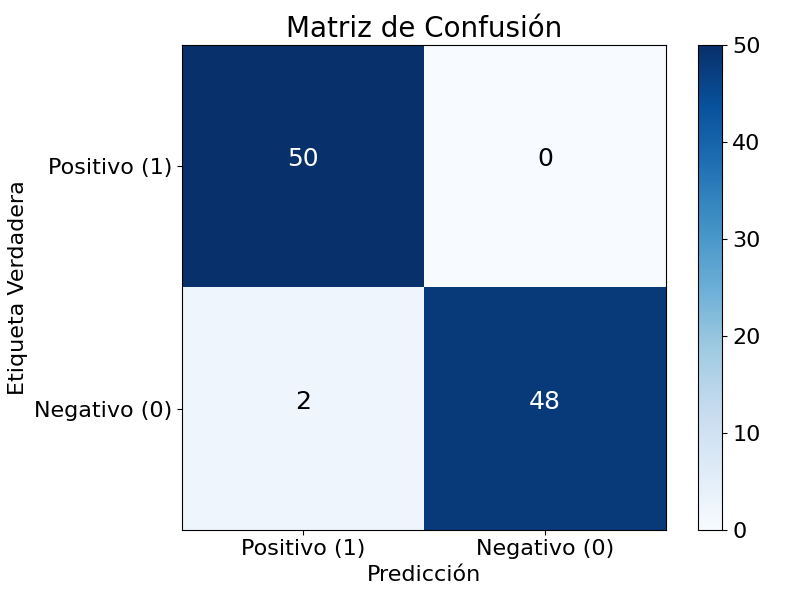
\includegraphics[width=0.48\textwidth]{training_plots/plot_architecture_3/confusion_matrix.png}
\caption{Matriz de Confusión generada tras probar la segunda Arquitectura.}
\label{fig:MatrizArqui2}
\end{figure}


Para la arquitectura 2 (ver cuadro ~\ref{tab:tiemposEjecucionComparacion}) el entrenamiento dura 771 segundos, y para las pruebas dura un total de 27.8 segundos. Por lo que por complejidad temporal es el segundo mejor, teniendo un rendimiento muy similar al anterior.

\begin{figure}[H]
\centering
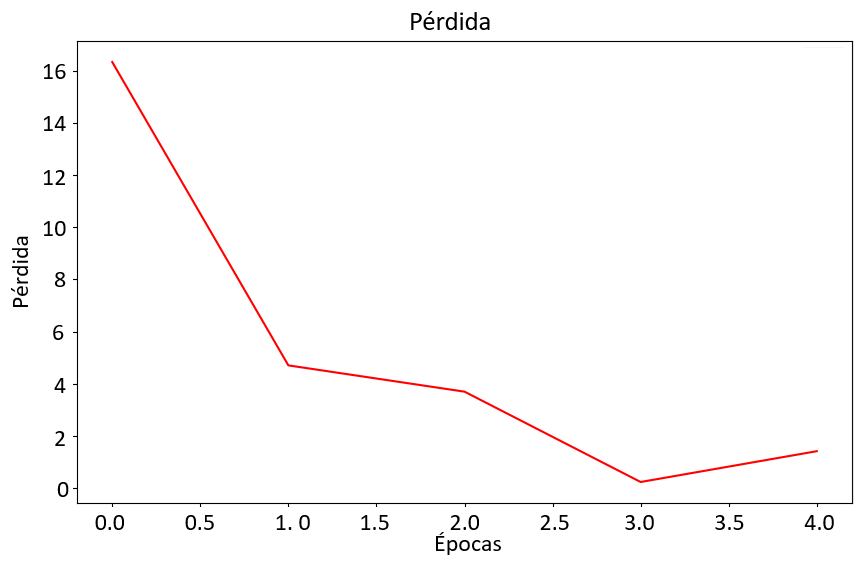
\includegraphics[width=0.48\textwidth]{training_plots/plot_architecture_3/loss_plot.png}
\caption{Grafo de pérdida generado durante el entrenamiento de nuestra segunda Arquitectura.}
\label{fig:perdidaArqui2}
\end{figure}


\begin{figure}[H]
\centering
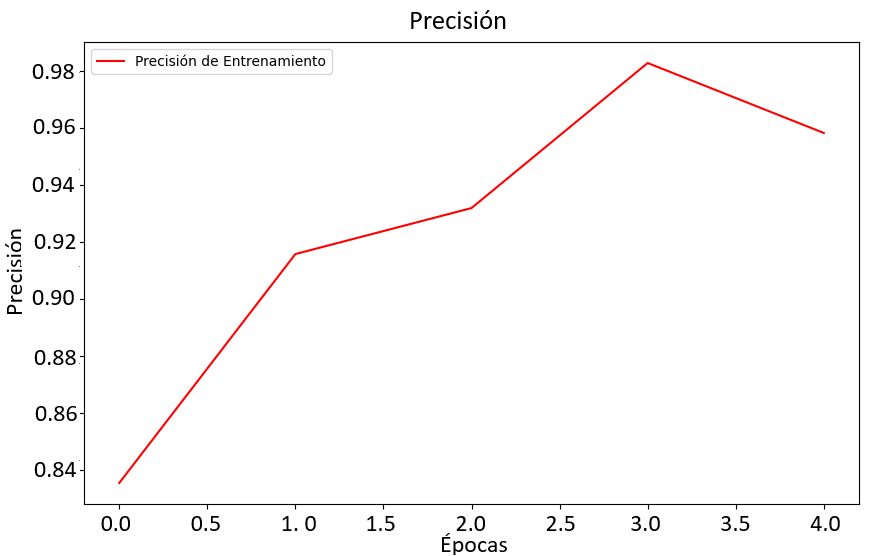
\includegraphics[width=0.48\textwidth]{training_plots/plot_architecture_3/precision_plot.png}
\caption{Grafo de precisión generado durante el entrenamiento de la segunda arquitectura propuesta.}
\label{fig:precisionArqui2}
\end{figure}


\begin{figure}[H]
\centering
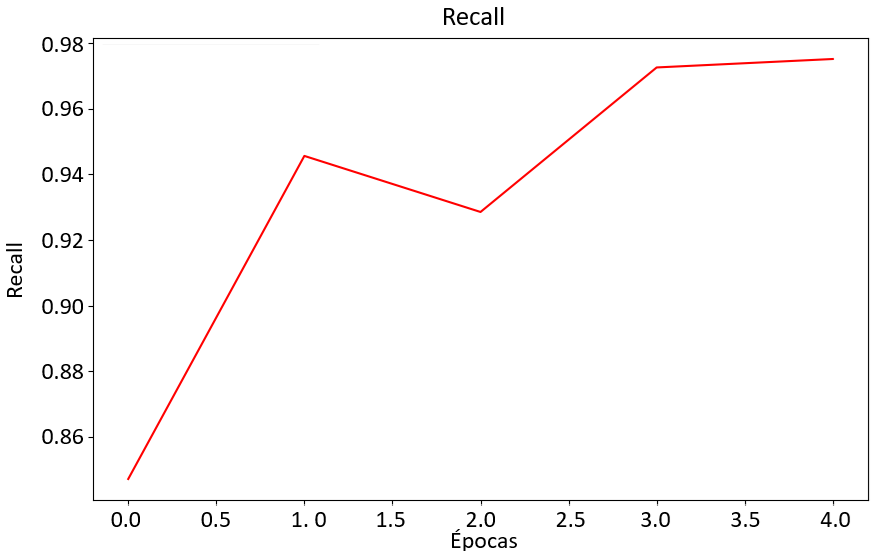
\includegraphics[width=0.48\textwidth]{training_plots/plot_architecture_3/recall_plot.png}
\caption{Grafo de recall generado durante el entrenamiento de la segunda arquitectura propuesta.}
\label{fig:recallArqui2}
\end{figure}

\begin{center}
    C. Arquitectura 3
\end{center}

Igual que los resultados anteriores, la matriz de confusión de la tercera arquitectura es casi perfecta, pero a diferencia de las anteriores, esta presenta 4 falsos negativos. 

\begin{figure}[H]
\centering
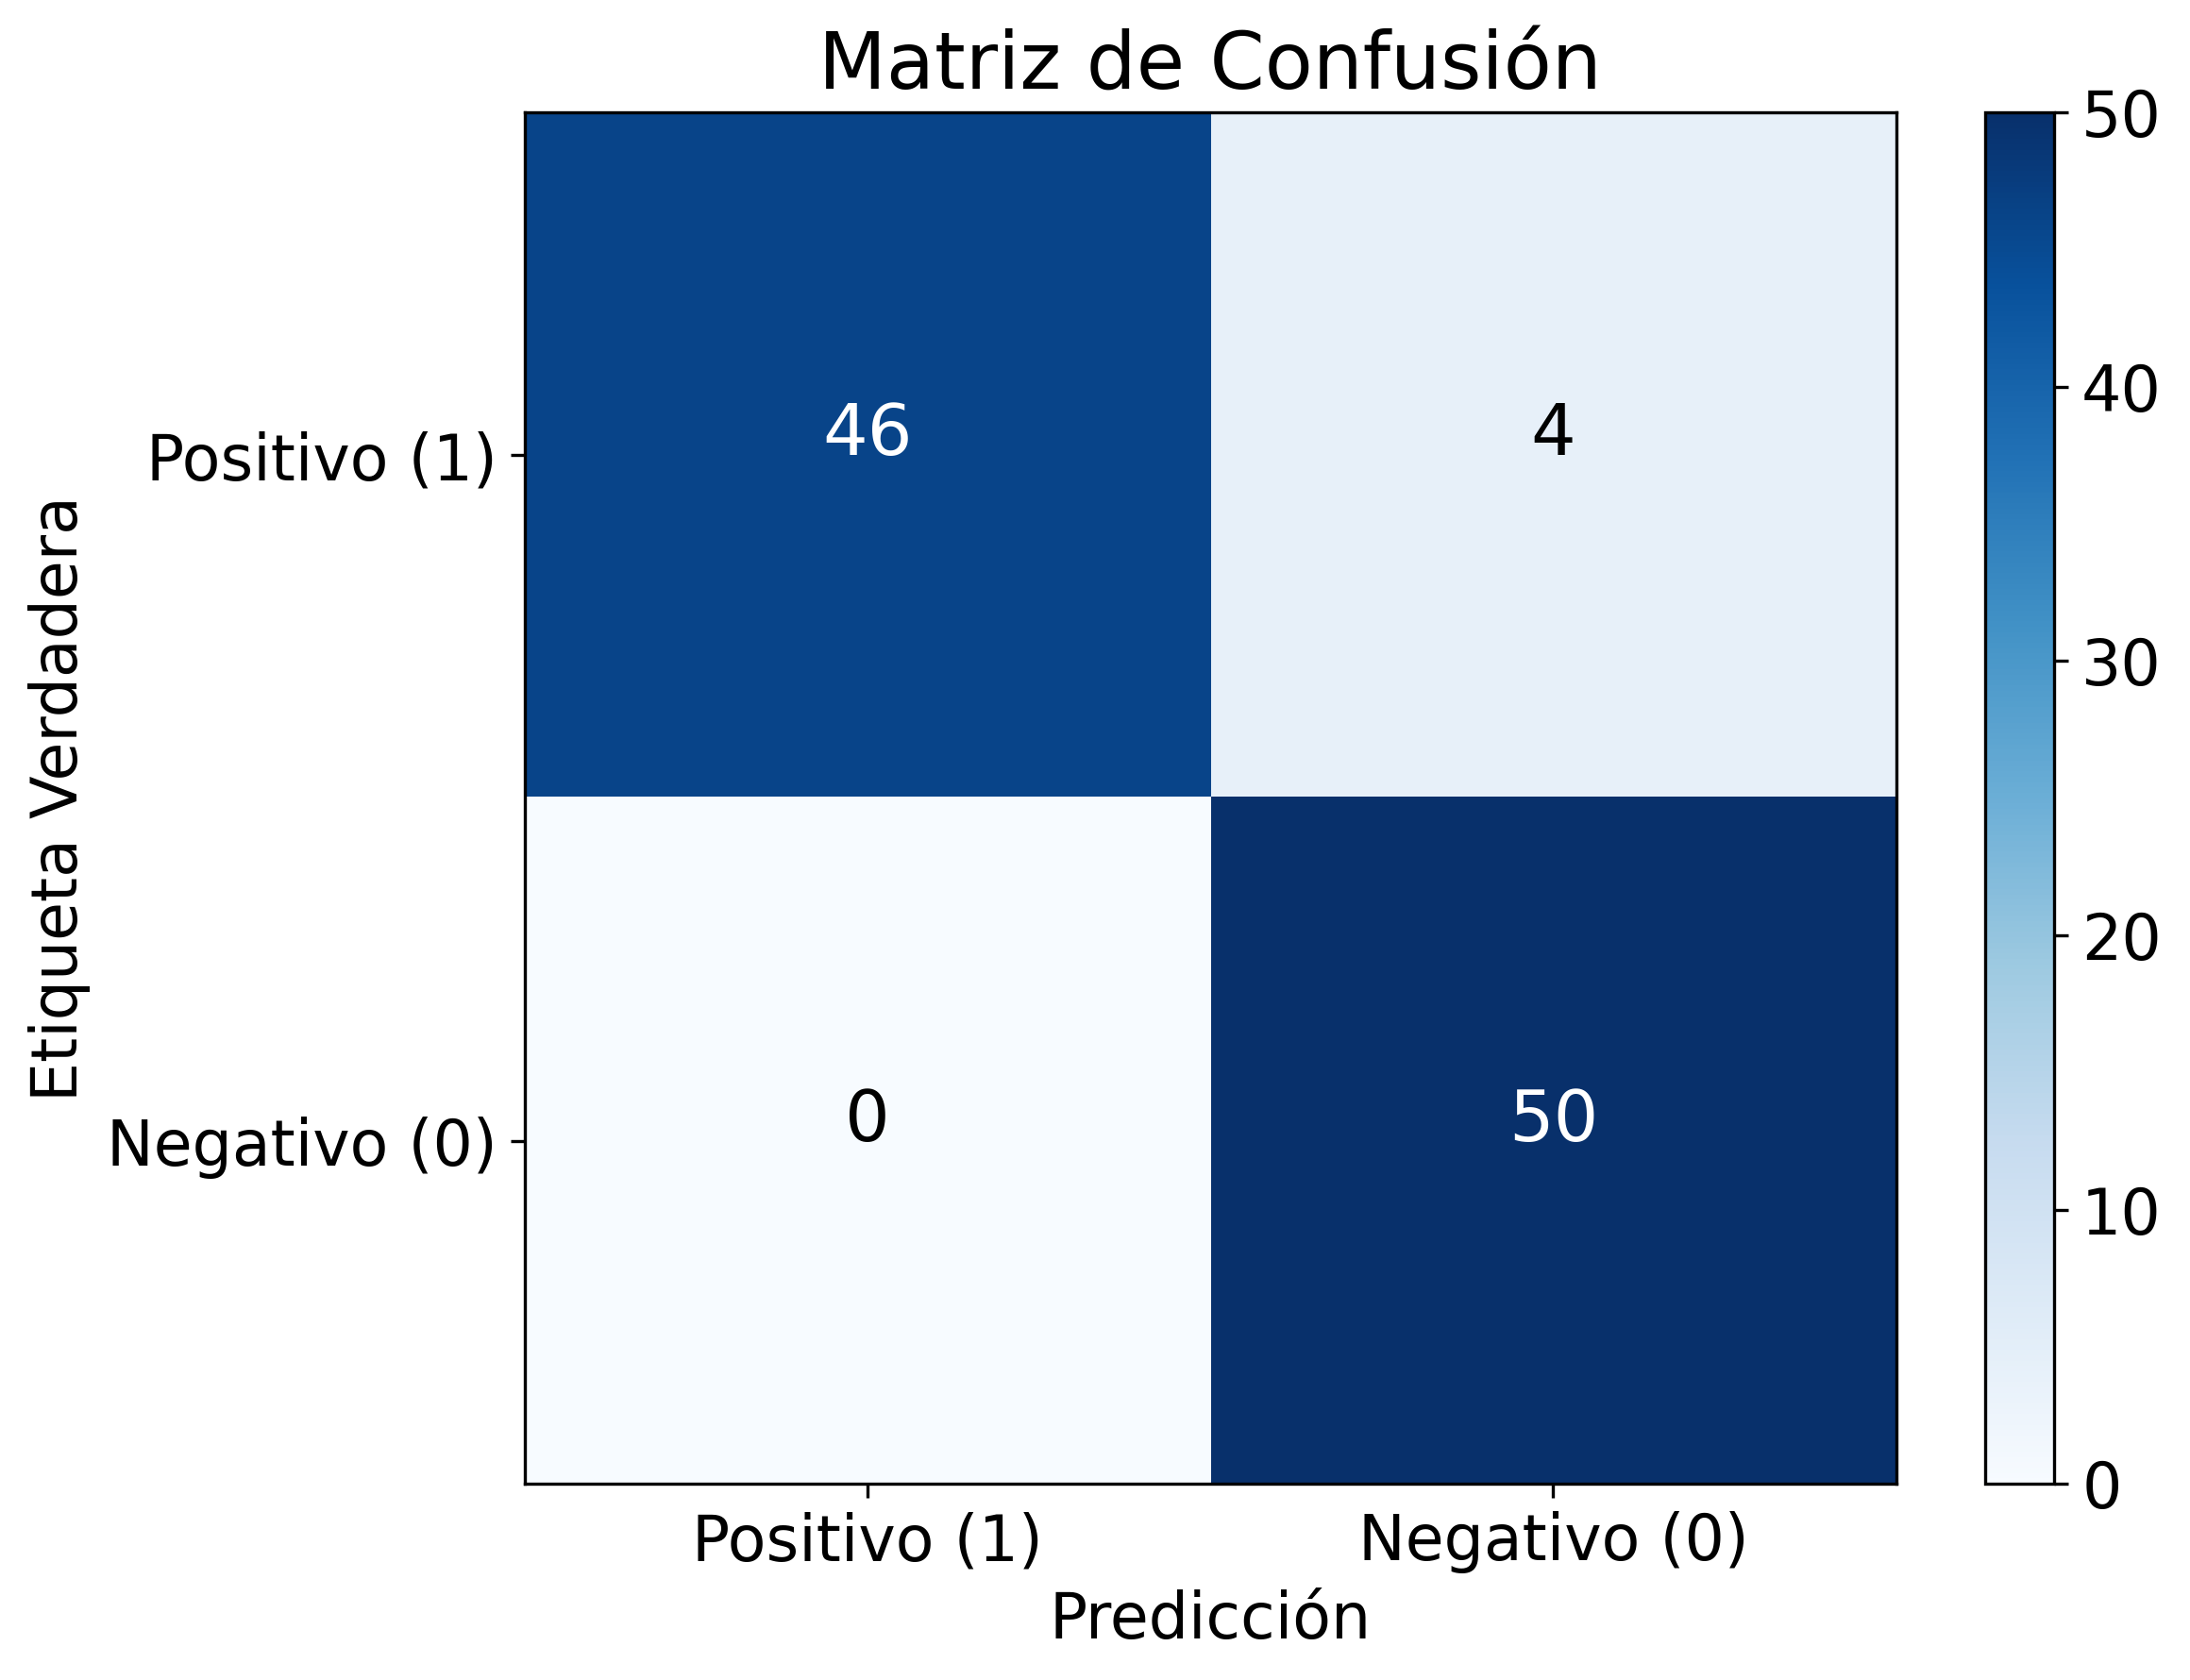
\includegraphics[width=0.48\textwidth]{training_plots/plot_architecture_4/confusion_matrix.png}
\caption{Matriz de Confusión generada tras probar la tercera arquitectura.}
\label{fig:MatrizArqui4}
\end{figure}


El entrenamiento con la arquitectura 3 dura 191 segundos, además para las pruebas dura un total de 21.7 segundos (ver cuadro ~\ref{tab:tiemposEjecucionComparacion}). Dado que el tiempo de entrenamiento es aproximadamente un cuarto del requerido por las otras implementaciones, se puede ajustar más parámetros e hiperparámetros sin consumir muchos recursos computacionales. En términos de complejidad temporal, esta implementación se presenta como la mejor opción propuesta.

\begin{figure}[H]
\centering
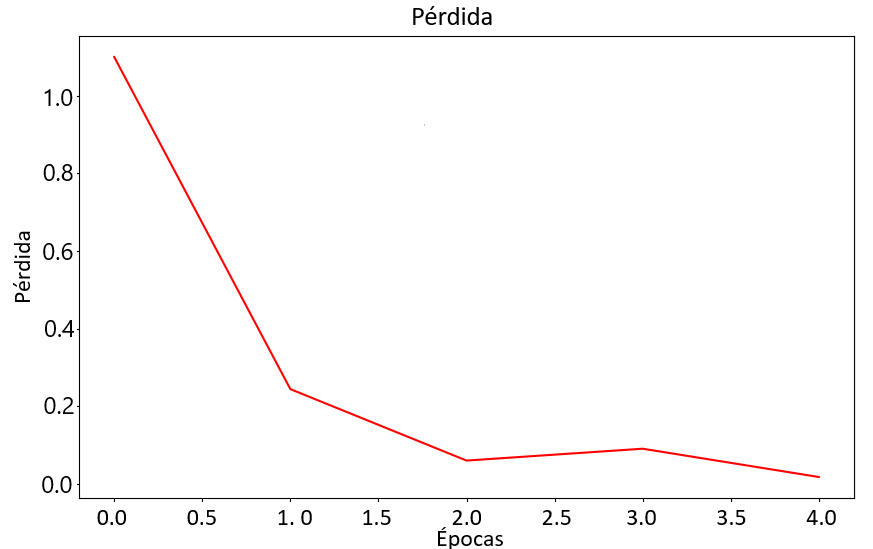
\includegraphics[width=0.48\textwidth]{training_plots/plot_architecture_4/loss_plot.png}
\caption{Grafo de pérdida generado durante el entrenamiento de la tercera arquitectura propuesta.}
\label{fig:perdidaArqui4}
\end{figure}


\begin{figure}[H]
\centering
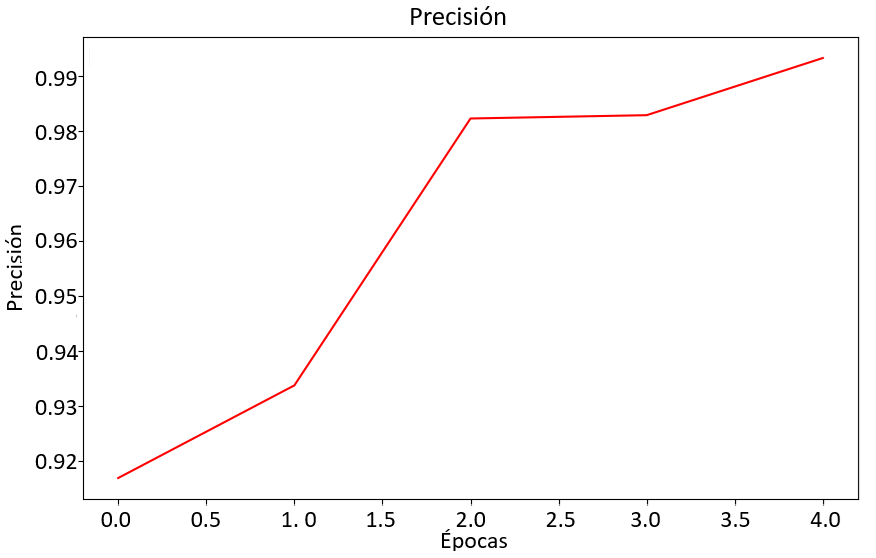
\includegraphics[width=0.48\textwidth]{training_plots/plot_architecture_4/precision_plot.png}
\caption{Grafo de precisión generado durante el entrenamiento de la tercera arquitectura propuesta.}
\label{fig:precisionArqui4}
\end{figure}


\begin{figure}[H]
\centering
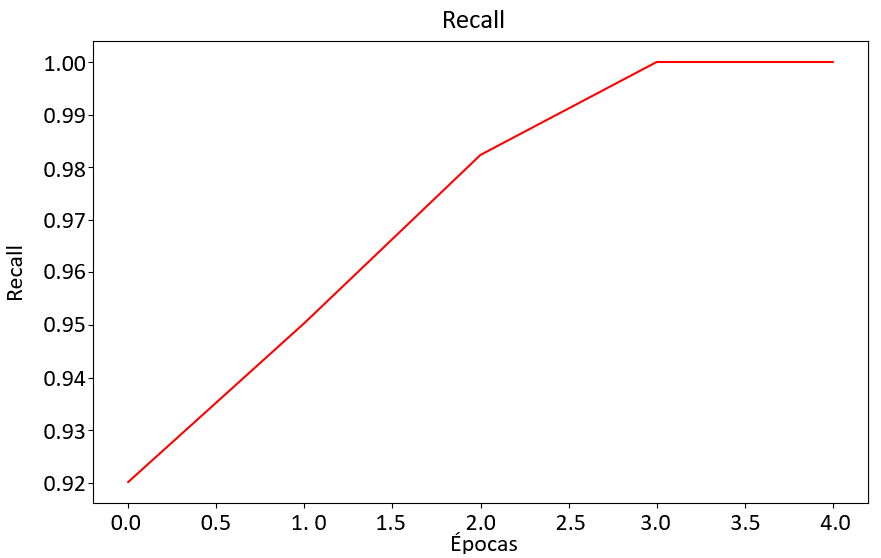
\includegraphics[width=0.48\textwidth]{training_plots/plot_architecture_4/recall_plot.png}
\caption{Grafo de recall generado durante el entrenamiento de la tercera arquitectura propuesta.}
\label{fig:recallArqui4}
\end{figure}

\section{Conclusiones}
A lo largo del desarrollo y tomando en cuenta los antecedentes, se ha demostrado que las CNN son altamente eficaces para identificar sonidos específicos de sirenas en entornos urbanos complejos. Esto no solo refuerza la precisión de estas redes en tareas de reconocimiento de audio, sino que también subraya su capacidad para ser adaptadas y optimizadas a contextos particulares, como el tráfico en San José, Costa Rica. Especialmente se denota la efectividad de la tercera arquitectura propuesta. Esta cuenta con una capa de MaxPooling, una capa de entrada, dos convolucionales con función de activación ReLu, seguido de una capa de aplanamiento.

Desde el marco teórico, el uso de redes neuronales convolucionales para el procesamiento de audio se ha consolidado como una técnica poderosa y versátil. La conversión de audios a espectrogramas ha permitido que las CNN identifiquen patrones acústicos complejos que son característicos de las sirenas de emergencia.

Los resultados obtenidos del proyecto responden directamente a los objetivos propuestos. En específico, se logró crear un modelo de detección de sirenas, por medio de las tres arquitecturas propuestas. Se evaluó el desempeño de estas y se definió la tercera como la preferida. Además de que se pudo crear un conjunto de datos a partir de recolecciones de campo y videos de internet para satisfacer las necesidades del modelo y el proyecto. Por lo que se logró la creación de un conjunto de datos específicos para el contexto costarricense y el desarrollo de arquitecturas de CNN optimizadas que permitieron alcanzar altos niveles de precisión en la detección de sirenas.

En conclusión, el proyecto establece una base para el uso de inteligencia artificial en la creación de sistemas de alerta para personas con discapacidad auditiva en Costa Rica. Por lo que las arquitecturas propuestas y la base de datos creada ofrecen resultados prometedores para usarlos y mejorarlos para futuras aplicaciones de la vida real. Para esto se recomienda, como mejoras del proyecto, hacer una recolección de datos más orientada al uso que se busca del sistema. Además de hacer una mayor investigación hacia las necesidades de las personas con discapacidades auditivas, serían los usuarios principales de este sistema. 

\appendices{}

\bibliographystyle{IEEEtran}
\bibliography{referencias}

\end{document}